\chapter{Supplementary Material}
\label{app:supplementary_figures}

This appendix collects per-experiment diagnostic plots, LSTM architecture
details, and additional tables supporting
Chapters~\ref{ch:rom_results} and~\ref{ch:wsindy_results}.

% -----------------------------------------------------------------------
\section{Additional density snapshots}
\label{sec:appE_snapshots}
% -----------------------------------------------------------------------

The following density-snapshot grids complement the representative gas
regime shown in Figure~\ref{fig:ch7_snapshots_gas} of the main text.

\begin{figure}[H]
\centering
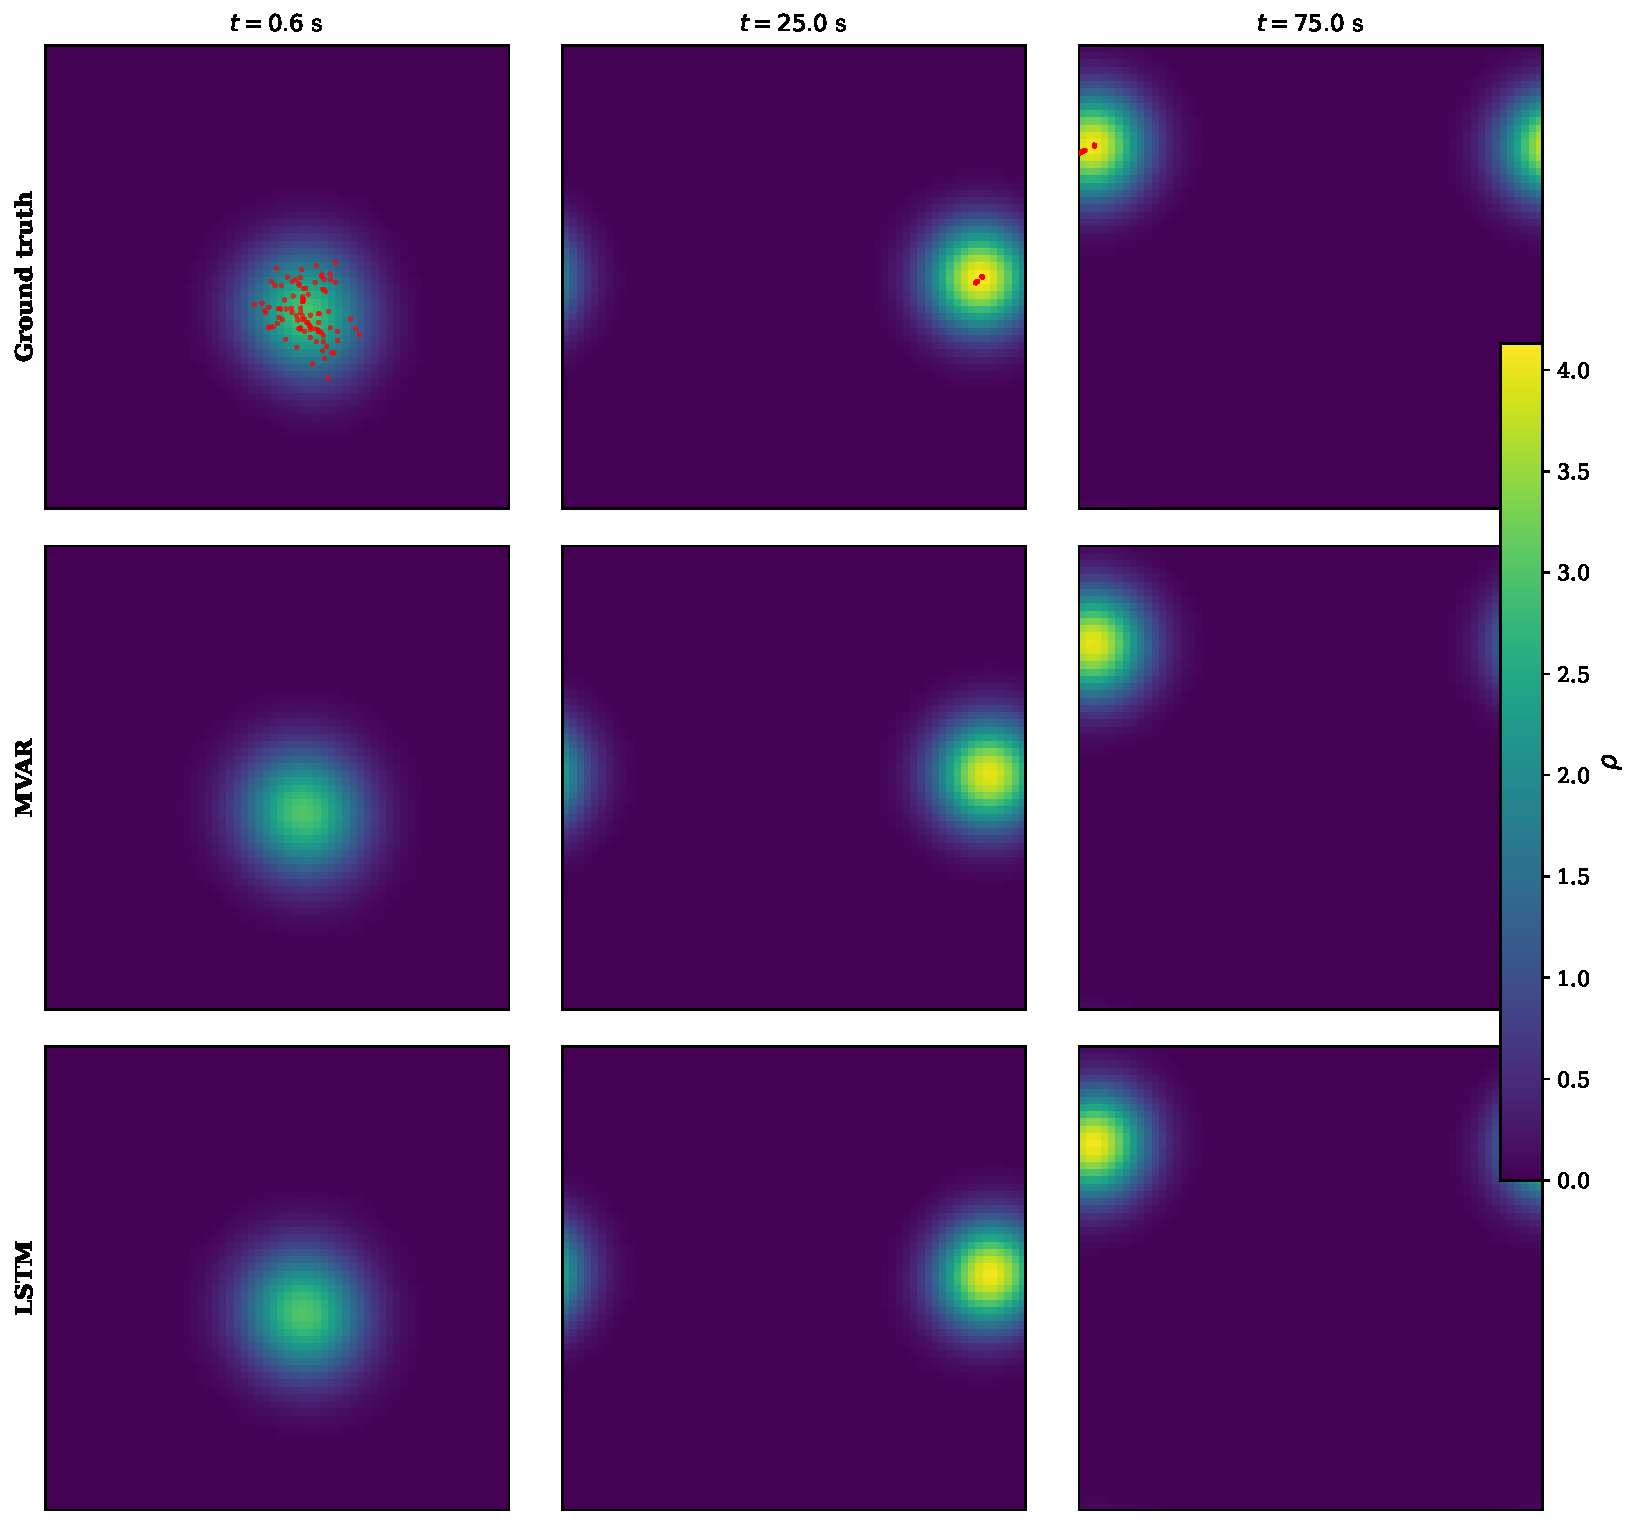
\includegraphics[width=0.92\textwidth]{../Thesis_Figures/appE_snapshots_blackhole.pdf}
\caption{Density snapshots truth vs.\ prediction for
\texttt{NDYN05\_blackhole} (Gaussian IC, test run~0).  Layout matches
Figure~\ref{fig:ch7_snapshots_gas}; rows show truth, MVAR, LSTM.}
\label{fig:appE_snapshots_blackhole}
\end{figure}

% -----------------------------------------------------------------------
\section{Eigenvalue spectra and stability}
\label{sec:appE_stability}
% -----------------------------------------------------------------------

The companion-matrix eigenvalue spectrum of the fitted MVAR model
reveals whether the linear surrogate is stable ($|\lambda|\le1$).
All nine benchmark regimes have spectral radius near or below unity;
regimes where one or more eigenvalues escape the unit circle required
clipping during forecast (Section~\ref{sec:ch7_mvar_failure}).

\begin{figure}[H]
\centering
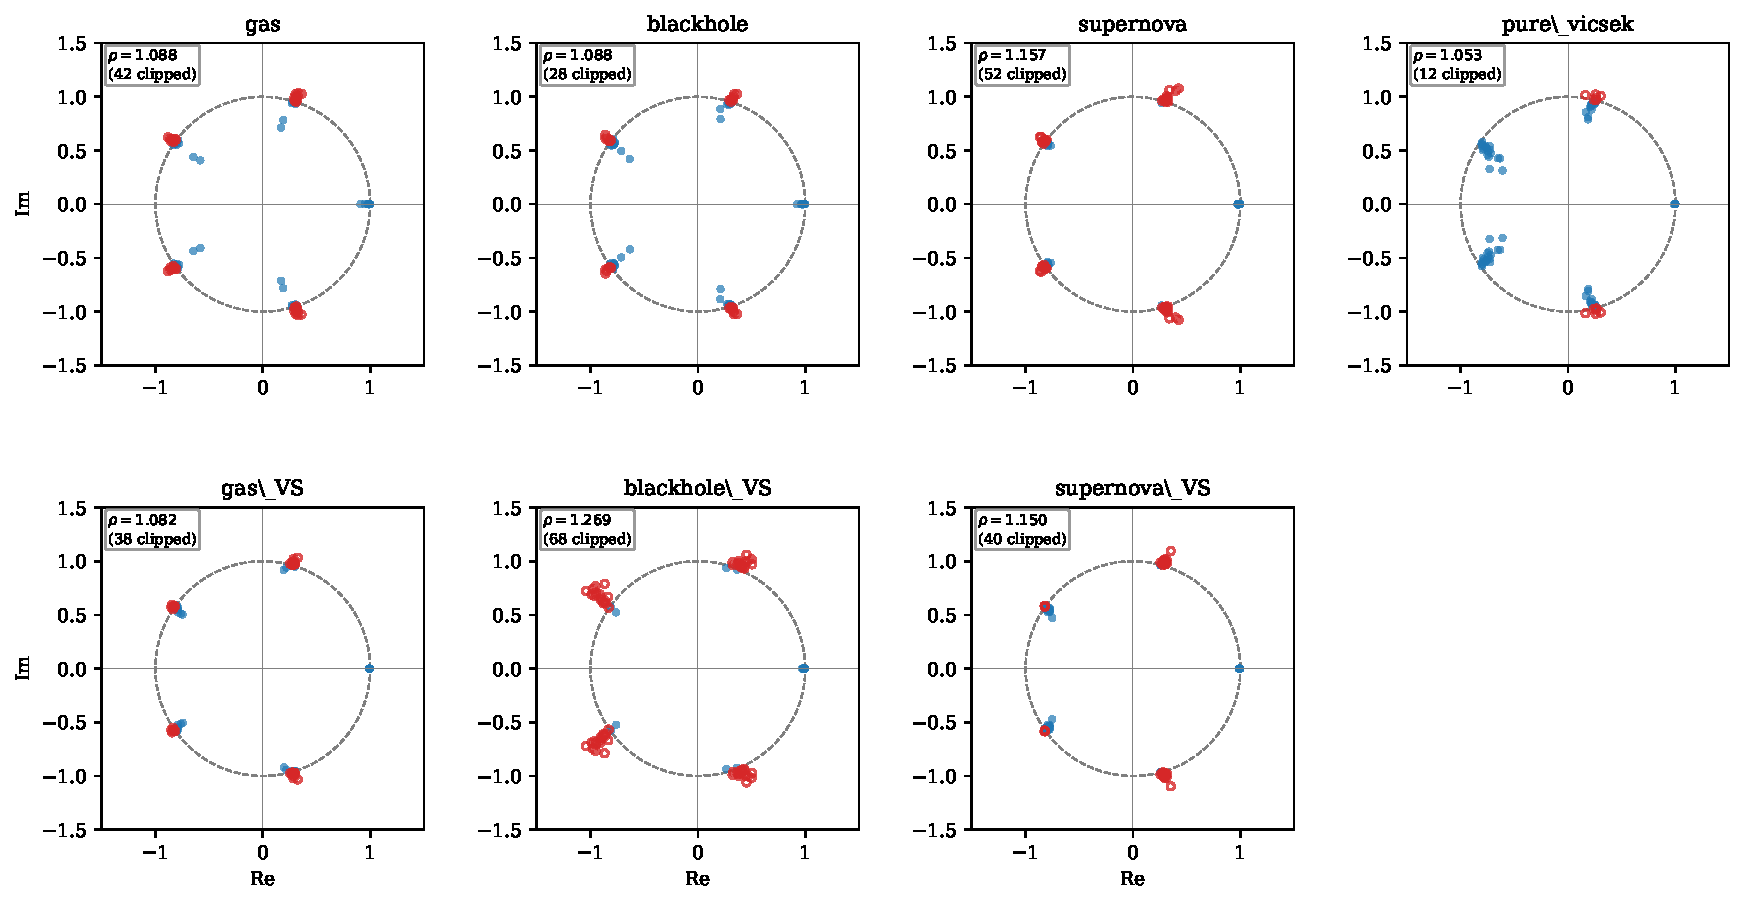
\includegraphics[width=\textwidth]{../Thesis_Figures/appE_eigenvalue_spectra.pdf}
\caption{Companion-matrix eigenvalue spectra for MVAR\@.  Eigenvalues
plotted in the complex plane (unit circle dashed).  Filled = stable;
open = clipped.  Spectral radius $\rho(\mathbf{A})$ annotated per panel.}
\label{fig:appE_stability}
\end{figure}

% -----------------------------------------------------------------------
\section{Per-experiment SVD decay}
% -----------------------------------------------------------------------

Figure~\ref{fig:appE_svd_decay_detail} compares the sPOD and standard
POD singular-value spectra per regime.  Regimes with stronger
translation symmetry (gas, blackhole) show the largest relative gain
from shift alignment, while near-stationary regimes (crystal) see
little difference.

\begin{figure}[H]
\centering
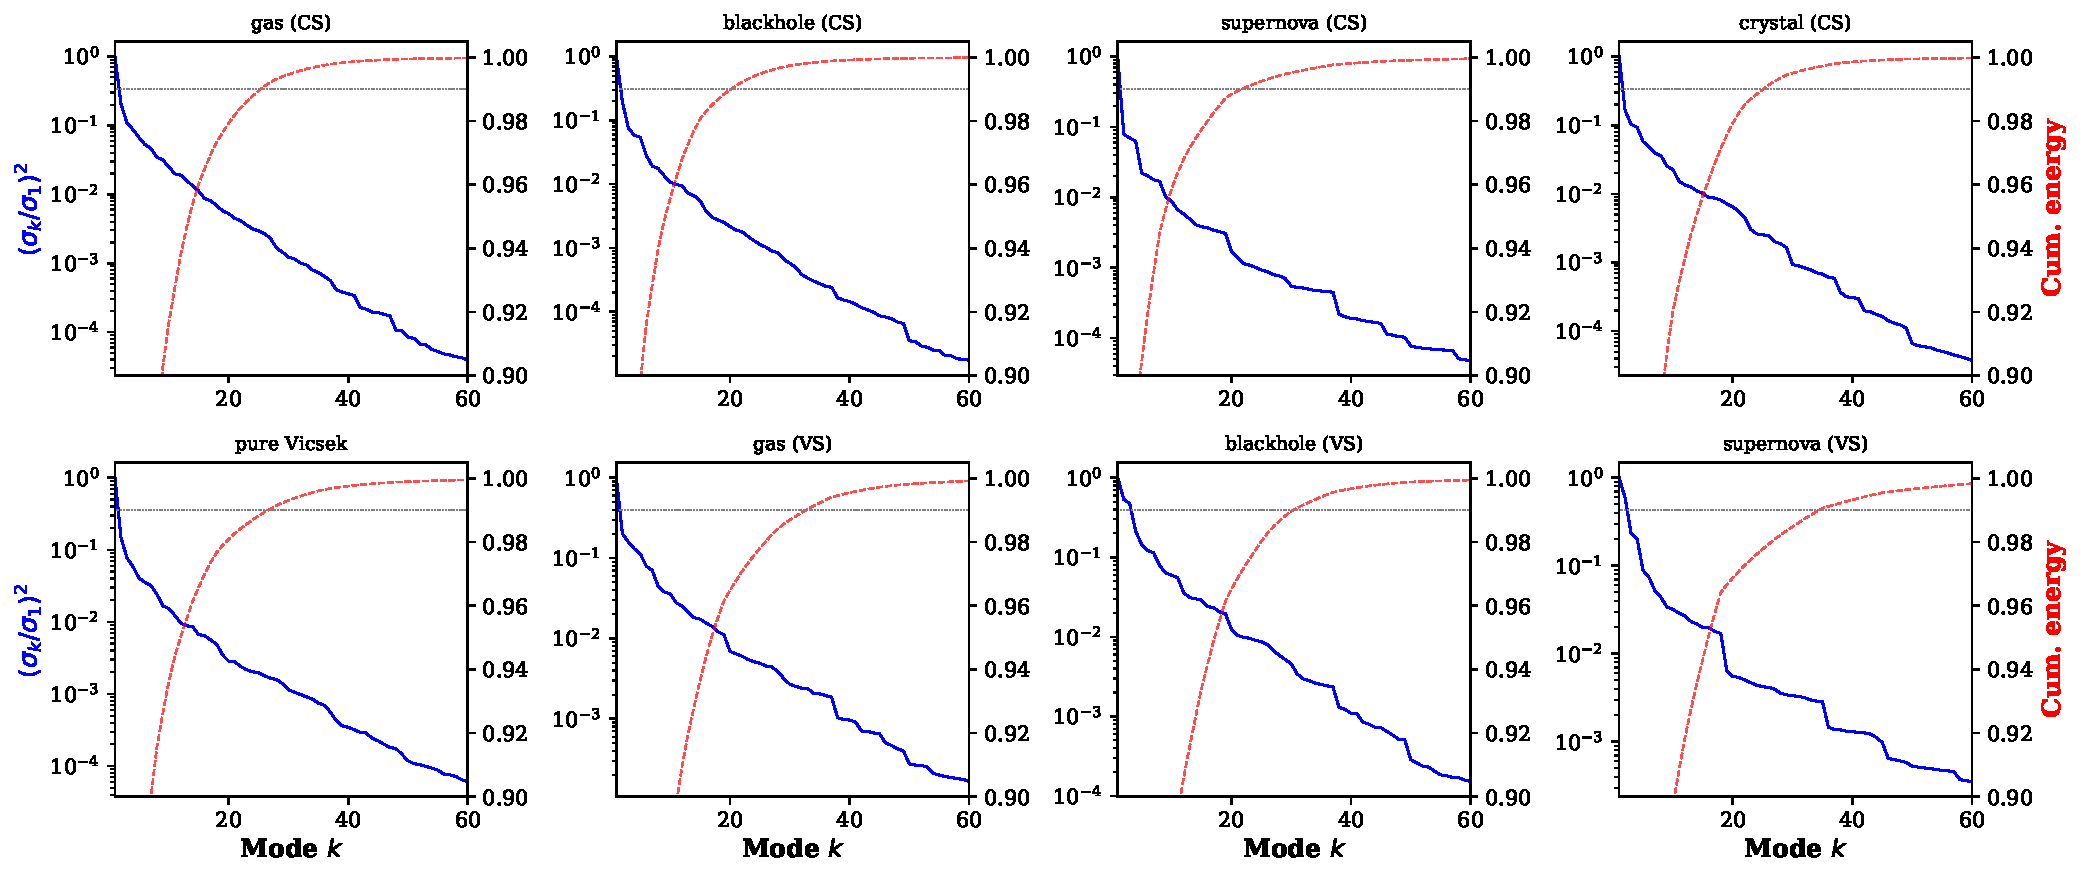
\includegraphics[width=0.95\textwidth]{../Thesis_Figures/thesis_svd_detail.pdf}
\caption{Per-experiment sPOD vs POD singular value spectra: normalised
eigenvalue decay (left) and cumulative energy (right).  Complements
Figure~\ref{fig:ch7_svd_decay}.}
\label{fig:appE_svd_decay_detail}
\end{figure}

% -----------------------------------------------------------------------
\section{Per-experiment $R^2$ degradation}
% -----------------------------------------------------------------------

Per-experiment $R^2(t)$ degradation curves for all nine benchmark regimes
are available in the full-catalogue Appendix~\ref{app:full_regime_catalogue}
(Figure~\ref{fig:appF_r2_degradation_combined}).
In summary, MVAR degrades most rapidly on supernova (fast spatial expansion),
while LSTM degrades most rapidly on variable-speed variants.

% -----------------------------------------------------------------------
\section{$R^2$ by regime group and density--latent comparison}
% -----------------------------------------------------------------------

Figure~\ref{fig:appE_r2_by_group} disaggregates the forecast $R^2$ by
regime group, confirming that MVAR dominates on CS regimes while LSTM
narrows the gap only for a few well-behaved VS cases.
Density-space and latent-space $R^2$ are closely aligned across all test
runs: the median absolute gap $|R^2_{\text{density}} - R^2_{\text{latent}}|$
is below $0.02$ for MVAR and $0.04$ for LSTM, confirming that the POD
truncation preserves forecast quality.

\begin{figure}[H]
\centering
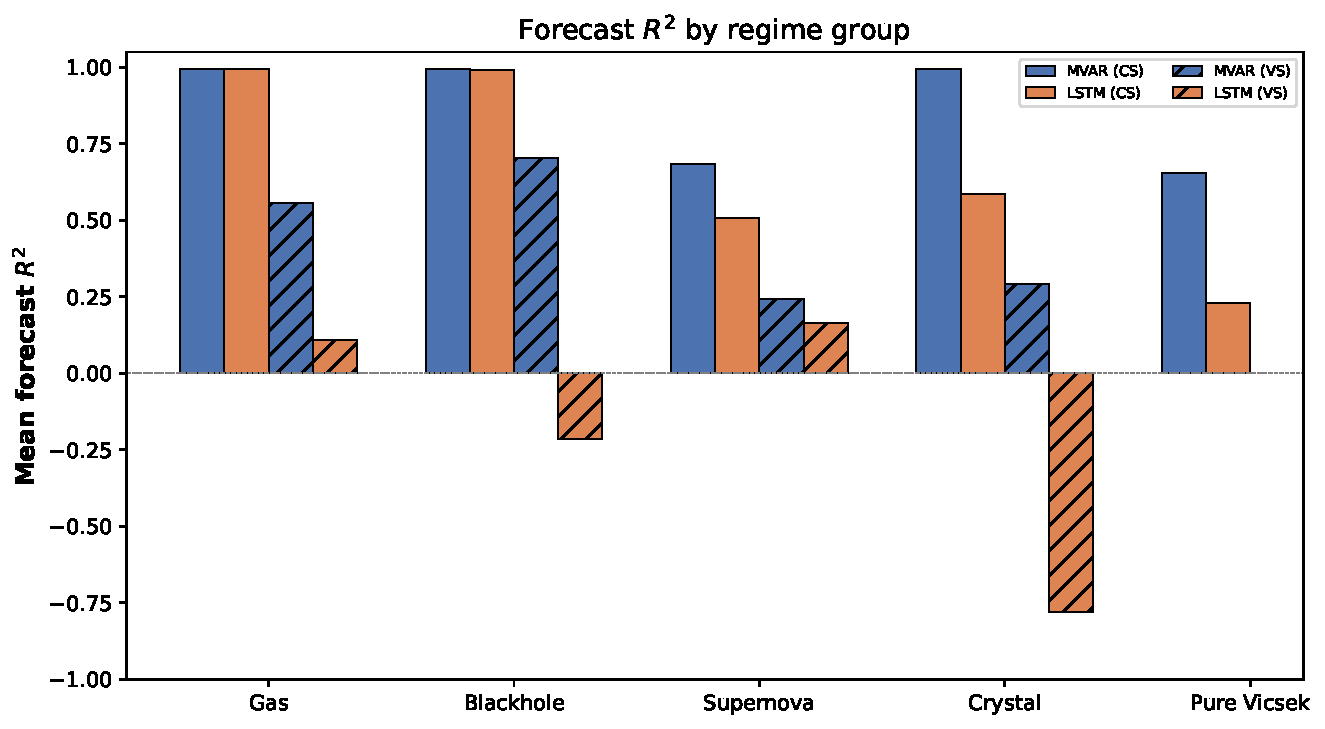
\includegraphics[width=0.88\textwidth]{../Thesis_Figures/thesis_r2_by_group.pdf}
\caption{Mean forecast $R^2$ by regime group (grouped bars: MVAR and
LSTM, constant-speed vs.\ variable-speed variants).  Complements
Figure~\ref{fig:ch7_r2_heatmap}.}
\label{fig:appE_r2_by_group}
\end{figure}

% -----------------------------------------------------------------------
\section{Mass conservation and phase dynamics}
% -----------------------------------------------------------------------

Both MVAR and LSTM preserve total mass to machine precision
($|M(t)/M_0 - 1| < 10^{-14}$) throughout the forecast horizon, since the
POD lifting step is a linear injection that exactly preserves the column
space of the snapshot matrix.
Figure~\ref{fig:appE_phase_dynamics} displays the shift-alignment
statistics aggregated across regimes.

\begin{figure}[H]
\centering
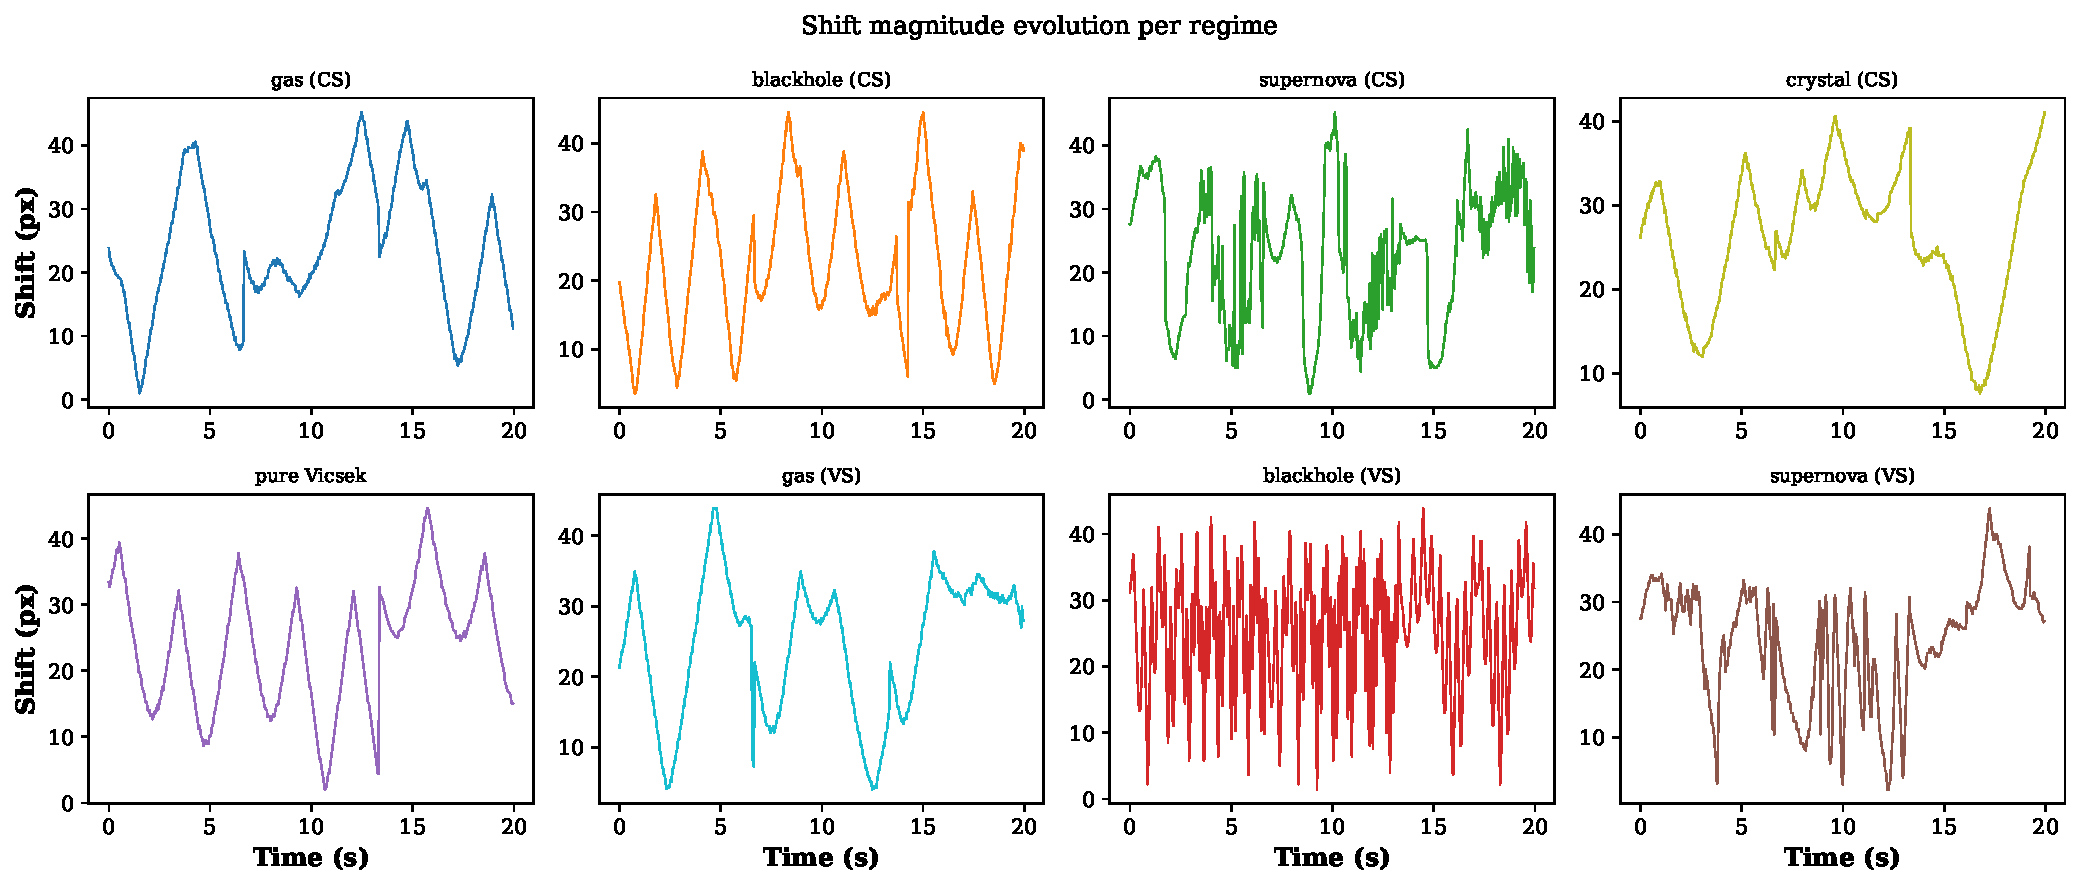
\includegraphics[width=\textwidth]{../Thesis_Figures/thesis_phase_dynamics_detail.pdf}
\caption{Aggregate phase (shift) dynamics: (a)~mean shift trajectory,
(b)~PSD, (c)~AR($p$) predictability, (d)~shift variance,
(e)~autocorrelation, (f)~legend.}
\label{fig:appE_phase_dynamics}
\end{figure}

% -----------------------------------------------------------------------
\section{Condition numbers}
% -----------------------------------------------------------------------

Among the $L^1$, $L^2$, and $L^\infty$ norms tracked over time for MVAR, the $L^\infty$ norm grows fastest, indicating that errors concentrate at density peaks.
Figure~\ref{fig:appE_condition_numbers} shows the condition number of the
weak-form design matrix; regimes with $\kappa>10^3$ exhibit wider
coefficient variability (cf.\ Table~\ref{tab:condition_numbers}).

\begin{figure}[H]
\centering
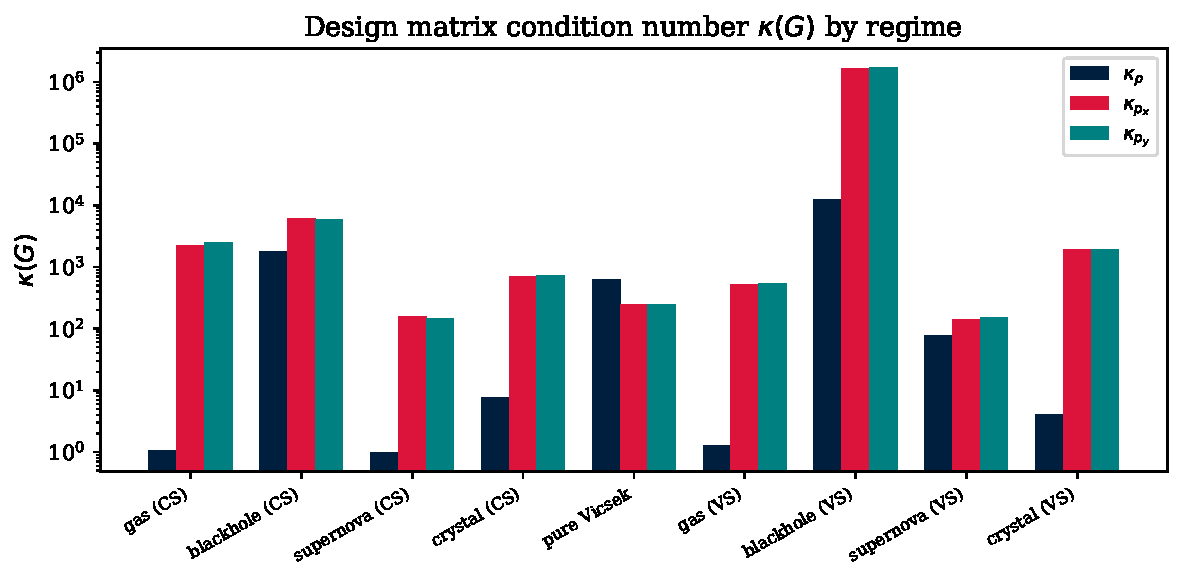
\includegraphics[width=0.88\textwidth]{../Thesis_Figures/thesis_condition_numbers.pdf}
\caption{Condition number $\kappa(G)$ of the weak-form design matrix,
grouped by regime and equation.  Log-scale $y$-axis.}
\label{fig:appE_condition_numbers}
\end{figure}

% -----------------------------------------------------------------------
\section{Representative WSINDy coefficient bar charts}
% -----------------------------------------------------------------------

The full coefficient profiles for all nine regimes are tabulated in
Tables~\ref{tab:wsindy_cross_rho}--\ref{tab:wsindy_cross_px}
(Chapter~\ref{ch:wsindy_results}).  The dominant-balance profile shifts
from diffusion-dominated (gas) to Morse-dominated (blackhole); the
variable-speed variants retain the same backbone terms but with larger
confidence intervals reflecting the noisier latent dynamics.

% -----------------------------------------------------------------------
\section{LSTM architecture and hyperparameters}
\label{sec:appG_lstm}
% -----------------------------------------------------------------------

The standard LSTM gate equations, referenced by Algorithm~\ref{alg:lstm_rom}, are:
\begin{align}
\mathbf{f}_\tau &= \sigma\!\bigl(\mathbf{W}_f[\mathbf{h}_{\tau-1},\mathbf{z}_\tau]+\mathbf{b}_f\bigr), &
\mathbf{i}_\tau &= \sigma\!\bigl(\mathbf{W}_i[\mathbf{h}_{\tau-1},\mathbf{z}_\tau]+\mathbf{b}_i\bigr), \nonumber\\
\mathbf{o}_\tau &= \sigma\!\bigl(\mathbf{W}_o[\mathbf{h}_{\tau-1},\mathbf{z}_\tau]+\mathbf{b}_o\bigr), &
\tilde{\mathbf{c}}_\tau &= \tanh\!\bigl(\mathbf{W}_c[\mathbf{h}_{\tau-1},\mathbf{z}_\tau]+\mathbf{b}_c\bigr), \nonumber\\
\mathbf{c}_\tau &= \mathbf{f}_\tau \odot \mathbf{c}_{\tau-1} + \mathbf{i}_\tau \odot \tilde{\mathbf{c}}_\tau, &
\mathbf{h}_\tau &= \mathbf{o}_\tau \odot \tanh(\mathbf{c}_\tau),
\label{eq:lstm_gates}
\end{align}
where $(\mathbf{h}_\tau,\mathbf{c}_\tau)$ are the hidden and cell states.

\begin{table}[H]
\centering\footnotesize
\caption{LSTM hyperparameters (final configuration).}
\label{tab:lstm_config}
\resizebox{0.65\textwidth}{!}{%
\begin{tabular}{lll}
\toprule
\textbf{Parameter} & \textbf{Config key} & \textbf{Value} \\
\midrule
Lag window          & \cv{lag}              & 5 (baseline) \\
Hidden units        & \cv{hidden\_units}    & 128 \\
LSTM layers         & \cv{num\_layers}      & 2   \\
Dropout (inter-layer) & \cv{dropout}        & 0.1 \\
Residual connection & \cv{residual}         & true \\
Layer normalisation & \cv{use\_layer\_norm} & true \\
Max epochs          & \cv{max\_epochs}      & 300 \\
Early-stop patience & \cv{patience}         & 40  \\
Learning rate       & \cv{lr}               & $7\times10^{-4}$ \\
Batch size          & \cv{batch\_size}      & 512 \\
Gradient clip       & \cv{grad\_clip}       & 5.0 \\
\bottomrule
\end{tabular}}%  end resizebox
\end{table}

% -----------------------------------------------------------------------
\section{Condition number table}
\label{sec:appG_condition}
% -----------------------------------------------------------------------

Table~\ref{tab:condition_numbers} lists $\kappa(\mathbf{G})$ for all nine
benchmark regimes.  The blackhole~VS regime has the highest condition
number ($\sim\!10^6$), consistent with its near-collinear library columns
and the wide confidence intervals observed in the bootstrap analysis
(Section~\ref{subsec:bootstrap}).

\begin{table}[H]
\centering\footnotesize
\caption{Condition number $\kappa(\mathbf{G})$ of the weak-form design
matrix per regime and target equation.  High~$\kappa$ indicates
near-collinearity, predicting wider coefficient variability across scales.}
\label{tab:condition_numbers}
\renewcommand{\arraystretch}{0.95}
\resizebox{0.65\textwidth}{!}{%
\begin{tabular}{llll}
\toprule
\textbf{Regime} & $\kappa(\mathbf{G}_{\rho})$ & $\kappa(\mathbf{G}_{p_x})$ & $\kappa(\mathbf{G}_{p_y})$ \\
\midrule
\texttt{NDYN04\_gas}          & $1.1$ & $2{,}259$ & $2{,}463$ \\
\texttt{NDYN05\_blackhole}    & $1{,}780$ & $6{,}012$ & $5{,}957$ \\
\texttt{NDYN06\_supernova}    & $1.0$ & $158$ & $144$ \\
\texttt{NDYN07\_crystal}      & $7.6$ & $703$ & $721$ \\
\texttt{NDYN08\_pure\_vicsek} & $623$ & $243$ & $246$ \\
\midrule
\texttt{NDYN04\_gas\_VS}       & $1.3$ & $527$ & $547$ \\
\texttt{NDYN05\_blackhole\_VS} & $12{,}496$ & $1.6{\times}10^6$ & $1.7{\times}10^6$ \\
\texttt{NDYN06\_supernova\_VS} & $77$ & $138$ & $152$ \\
\texttt{NDYN07\_crystal\_VS}   & $4.0$ & $1{,}917$ & $1{,}935$ \\
\bottomrule
\end{tabular}}%  end resizebox
\end{table}
